% A first spacetime diagram: worldlines of a particle at rest, a particle moving
% at speed 0.4, a particle that speeds up and slows down, and light (c = 1).
\documentclass[tikz,border=1pt]{standalone}
% Shared preamble for the standalone figures: the book's fonts, palette and
% drawing styles. Figures are drawn at their final printed size. A column is
% 3.35in (241pt) wide; a figure across both columns is 7in (505pt) wide.

\usepackage[T1]{fontenc}
\usepackage{newpxtext}
\usepackage[varbb]{newpxmath}
\usepackage[semibold,scale=0.95,lining]{sourcesanspro}
\usepackage{xcolor}
% Palette shared by the book and by the standalone figures in figures/src.
% One main hue (blue), one accent (orange), and a few roles used sparingly.

\definecolor{seblue}{HTML}{1D5B8F}    % headings, worked examples, main curves
\definecolor{seblueDark}{HTML}{123E63}
\definecolor{seorange}{HTML}{DC7A26}  % thought experiments, light and light cones
\definecolor{seteal}{HTML}{1F8577}    % checks, travellers and ships
\definecolor{sered}{HTML}{C0392B}     % negative energy, tension, violations
\definecolor{seviolet}{HTML}{5E548E}  % going deeper
\definecolor{sesand}{HTML}{8C6A3F}    % history
\definecolor{segray}{HTML}{6B7480}    % axes, guides, secondary labels
\definecolor{selight}{HTML}{D5DAE1}   % grids and faint rules

\usepackage{siunitx}
\usepackage{fontawesome5}
\usepackage{tikz}
\usetikzlibrary{arrows.meta,calc,positioning,decorations.pathreplacing,
  decorations.markings,shapes.geometric,fadings,shadings,patterns,3d,
  intersections,backgrounds}
\usepackage{pgfplots}
\pgfplotsset{compat=1.18}
\usepgfplotslibrary{fillbetween,groupplots,colormaps}

\tikzset{
  >={Latex[length=2.1mm,width=1.4mm]},
  every picture/.style={line cap=round, line join=round},
  lbl/.style={font=\sffamily\footnotesize, text=black!85},
  smalllbl/.style={font=\sffamily\scriptsize, text=black!75},
  guide/.style={segray, line width=0.4pt},
  axisline/.style={segray, line width=0.5pt, -{Latex[length=1.7mm,width=1.1mm]}},
  light/.style={seorange, line width=0.9pt},
  lightdash/.style={seorange, line width=0.9pt, dash pattern=on 3pt off 2pt},
  ship/.style={seteal, line width=1.4pt},
  cone/.style={fill=seorange!22, draw=seorange!85!black, line width=0.35pt},
}

\pgfplotsset{
  se axis/.style={
    axis lines=left,
    axis line style={segray, line width=0.5pt, -{Latex[length=1.6mm,width=1.1mm]}},
    tick style={segray, line width=0.4pt},
    major tick length=2.5pt,
    tick label style={font=\sffamily\scriptsize, text=black!75},
    label style={font=\sffamily\footnotesize, text=black!85},
    every axis plot/.append style={line width=1.1pt},
    legend style={font=\sffamily\scriptsize, draw=none, fill=none},
    scaled ticks=false,
    xticklabel={\sansnum{\tick}}, yticklabel={\sansnum{\tick}},
  },
}

% Numbers in figures are set in the sans-serif text font, with a true minus.
\sisetup{mode=text, reset-text-family=false, reset-text-series=false,
  reset-text-shape=false, drop-zero-decimal, group-minimum-digits=5}
% Tick values arrive as long decimals (1.5000000000); parse them first.
\newcommand{\sansnum}[1]{\begingroup\pgfkeys{/pgf/fpu=false}%
  \pgfmathparse{1*(#1)}\num{\pgfmathresult}\endgroup}

\begin{document}
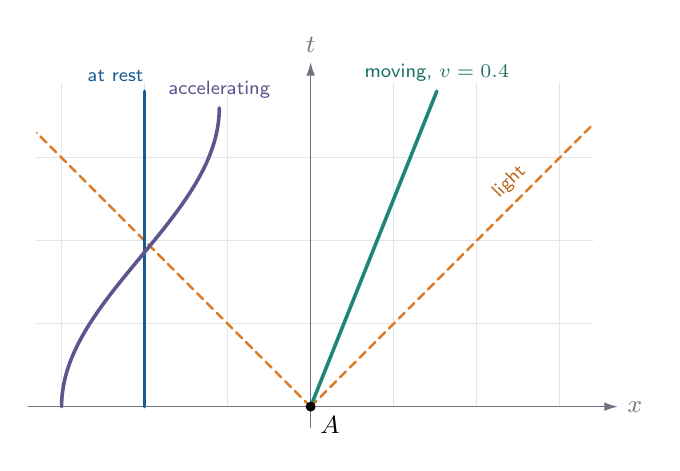
\begin{tikzpicture}[x=30pt, y=30pt]
% faint grid
\foreach \x in {-3,...,3} \draw[selight!70, line width=0.3pt] (\x,0) -- (\x,3.9);
\foreach \t in {1,...,3} \draw[selight!70, line width=0.3pt] (-3.3,\t) -- (3.4,\t);
\draw[axisline] (-3.4,0) -- (3.7,0) node[anchor=west, font=\small] {$x$};
\draw[axisline] (0,-0.25) -- (0,4.15) node[anchor=south, font=\small] {$t$};
% light from A
\draw[lightdash] (0,0) -- (3.4,3.4);
\draw[lightdash] (0,0) -- (-3.3,3.3);
\node[smalllbl, text=seorange!85!black, rotate=45, anchor=south] at (2.55,2.55) {light};
% at rest
\draw[seblue, line width=1.3pt] (-2,0) -- (-2,3.8);
\node[smalllbl, anchor=south, text=seblue] at (-2.35,3.8) {at rest};
% moving at 0.4
\draw[seteal, line width=1.3pt] (0,0) -- (1.52,3.8);
\node[smalllbl, anchor=south, text=seteal!85!black] at (1.52,3.8) {moving, $v = 0.4$};
% speeding up then slowing down: x(t) = -3 + 1.9 (1 - cos(pi t/3.6))/2,
% whose largest speed is 1.9 pi/7.2 = 0.83, below the speed of light
\draw[seviolet, line width=1.3pt, domain=0:3.6, samples=60, variable=\t]
  plot ({-3 + 0.95*(1 - cos(180*\t/3.6))}, {\t});
\node[smalllbl, anchor=south, text=seviolet] at (-1.1,3.6) {accelerating};
\fill (0,0) circle (1.8pt) node[anchor=north west, font=\small] {$A$};
\end{tikzpicture}
\end{document}
